\subsection{Example: Initial Condition and Rate of Something Decaying}\label{ex:decay-set-sample-accuracy}

TK - if we keep this example, I need to write about it.

\emph{Why is it here?}
Because I can. LOL. No, but seriously...
Whereas the truth was impacting our choice of optimal spatial location for measurements in the previous example, we now find that measuring at different points in time changes our inverse density as well, and should be taken into consideration for optimal experimental design purposes.

\begin{figure}[h]
\begin{minipage}{.4\textwidth}
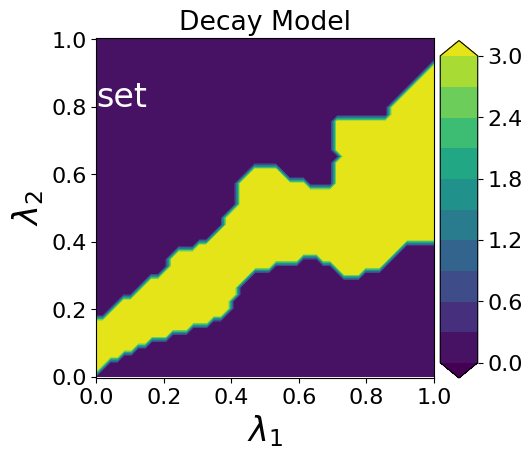
\includegraphics[width=\linewidth]{examples/fig_decay_q1/DecayModel--set_N50_em.png}
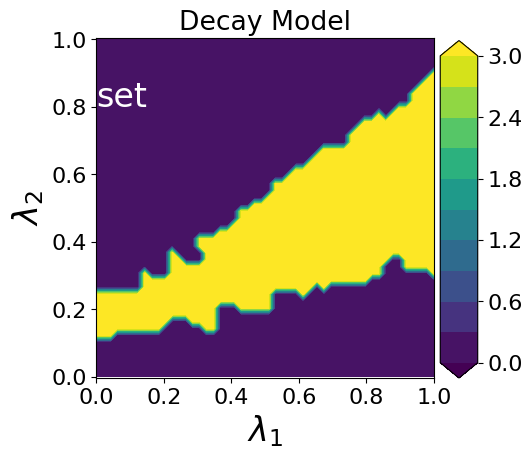
\includegraphics[width=\linewidth]{examples/fig_decay_q1/DecayModel--set_N500_em.png}

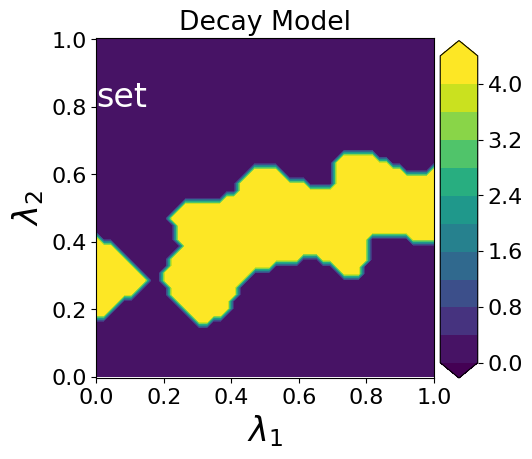
\includegraphics[width=\linewidth]{examples/fig_decay_q2/DecayModel--set_N50_em.png}
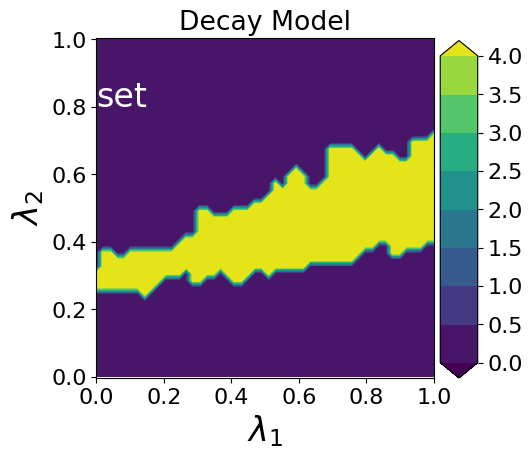
\includegraphics[width=\linewidth]{examples/fig_decay_q2/DecayModel--set_N500_em.png}
\end{minipage}
\begin{minipage}{.4\textwidth}
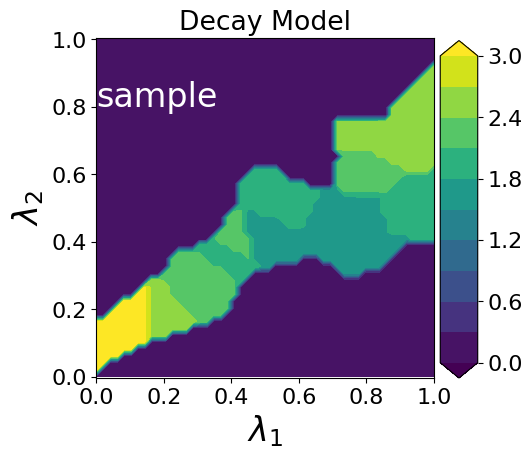
\includegraphics[width=\linewidth]{examples/fig_decay_q1/DecayModel--sample_N50_mc.png}
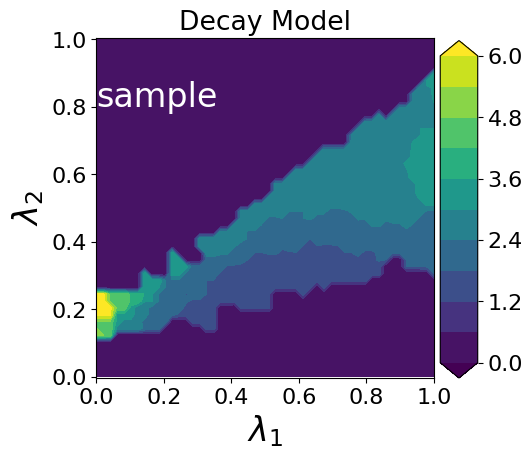
\includegraphics[width=\linewidth]{examples/fig_decay_q1/DecayModel--sample_N500_mc.png}

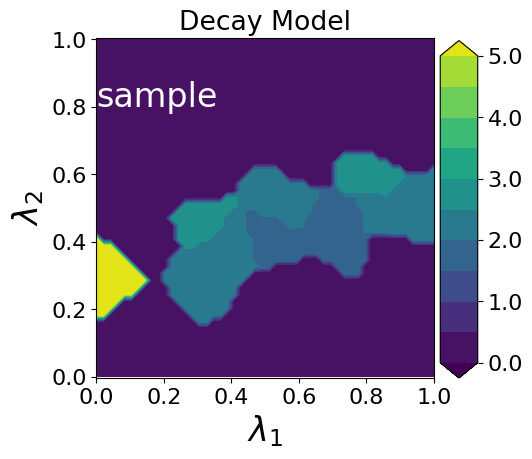
\includegraphics[width=\linewidth]{examples/fig_decay_q2/DecayModel--sample_N50_mc.png}
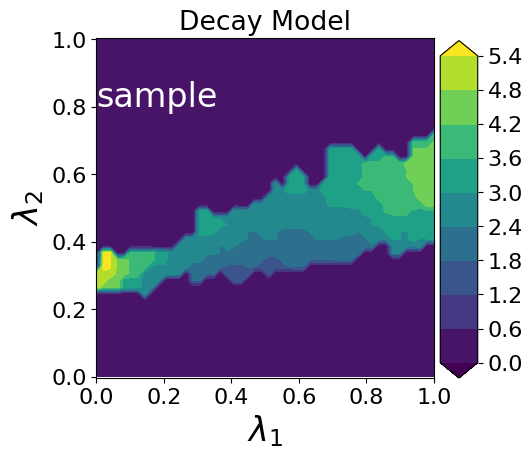
\includegraphics[width=\linewidth]{examples/fig_decay_q2/DecayModel--sample_N500_mc.png}
\end{minipage}

\caption{The inverse image of the reference measure for $\qoiA$ (top half) and $\qoiB$ (bottom half). }
\label{fig:decay-convergence}
\end{figure}

In the nonlinear examples, the location of the true parameter value has just as much of an impact on our ability to recover an inverse density as does the map we use (induced by where or when we measure).
However, we cannot know the location of the parameters that led to our observations ahead of time, so the best we can hope to do is pick maps that perform well ``on average,'' which may seem a bit dis-satisfactory if it means leaving out data that has already been collected.
In situations where the decision of where/when to measure needs to be made, there is no getting around needing to make decisions based on the average skewness of the operator, but when data has already been collected, we have several options at our disposal.

For instance, we may look into solving a series of inverse problems, passing the updated solution from one as the initial density to the next, choosing different QoI maps each time from the available data.
We explore this in \ref{sec:ch05-sequential} with respect to the MUD point, but leave exploration of the full densities being iterated for future work.
Another approach would be to construct a piecewise-defined QoI map, where maps can be used in locally-optimal ways to create globally-optimal geometric properties from the contributions of the individuals components.
[TK - we have work like this... but we should just leave it to future work since it's some time to clean it up for presentation... ]
